\chapter{Euler and Hamilton}

\section{Euler}
% Imagine (Unnumbered Header)
\par\vspace{0.5cm}\noindent
\needspace{3\baselineskip}
{\large \underline{\textbf{Imagine}}}
\par\vspace{0.2cm}
A salesperson with their wagon wants to pass by every street in his neighbourhood to sell their goods. Of course, they want to minimize efforts, so they would like to avoid passing the same street twice. These type of problems are considered when discussing \textbf{\color{red}Eulerian graphs}.

Then, as only few people buy, they switch to their car and only visit a central place in each city of the area. Again, to improve efficiency, they only want to visit each city once. This type of problem is studied when discussing \textbf{\color{red}Hamiltonian graphs}.

How do these two problems differ? Let's find out!

% 4.1 Definition
\begin{definition}
We call a trail in a graph $G$ an \textbf{\color{red}Eulerian trail} if it contains every edge of $G$. We call it an \textbf{\color{red}Eulerian circuit} if it is a closed Eulerian trail. Finally, the graph $G$ itself is called an \textbf{\color{red}Eulerian graph} iff it contains an Eulerian circuit.
\end{definition}

% 4.2 Examples
\begin{example}
\begin{enumerate}
    \item[1)]
    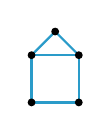
\begin{tikzpicture}[scale=0.6, baseline=(current bounding box.center)]
        \coordinate (a) at (0,0); \coordinate (b) at (1,0);
        \coordinate (c) at (1,1); \coordinate (d) at (0,1);
        \coordinate (e) at (0.5,1.5);
        \draw[cyan!80!black, thick] (a)--(b)--(c)--(d)--(a);
        \draw[cyan!80!black, thick] (d)--(e)--(c);
        \foreach \p in {a,b,c,d,e} \filldraw (\p) circle (2pt);
    \end{tikzpicture}
    \textbf{\color{blue}is not} Eulerian, but has an Eulerian trail.

    \item[2)]
    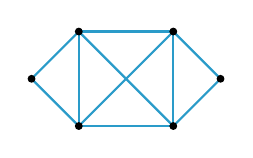
\begin{tikzpicture}[scale=0.6, baseline=(current bounding box.center)]
        % Left node, Central Box, Right node
        \coordinate (l) at (-2,0);
        \coordinate (tl) at (-1,1);
        \coordinate (bl) at (-1,-1);
        \coordinate (tr) at (1,1);
        \coordinate (br) at (1,-1);
        \coordinate (r) at (2,0);

        % Wings
        \draw[cyan!80!black, thick] (l)--(tl);
        \draw[cyan!80!black, thick] (l)--(bl);
        \draw[cyan!80!black, thick] (r)--(tr);
        \draw[cyan!80!black, thick] (r)--(br);

        % Central K4
        \draw[cyan!80!black, thick] (tl)--(tr)--(br)--(bl)--(tl); % Outer Box
        \draw[cyan!80!black, thick] (tl)--(br); % Diagonal
        \draw[cyan!80!black, thick] (bl)--(tr); % Diagonal

        \foreach \p in {l,tl,bl,tr,br,r} \filldraw (\p) circle (2pt);
    \end{tikzpicture}
    \textbf{\color{green!60!black}is indeed} Eulerian.

    \item[3)] Any cycle $C_n$ is clearly Eulerian.
    
    \item[4)] Any path of length $n \ge 1$ is \textbf{\color{red}not} Eulerian but has an Eulerian trail.

    \item[5)]
    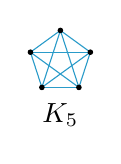
\begin{tikzpicture}[scale=0.4, baseline=(current bounding box.center)]
        \foreach \i in {1,...,5} \coordinate (v\i) at (90+72*\i:1);
        \foreach \i in {1,...,5} \foreach \j in {\i,...,5} \draw[cyan!80!black] (v\i)--(v\j);
        \foreach \i in {1,...,5} \filldraw (v\i) circle (2pt);
        \node[below] at (0,-1) {$K_5$};
    \end{tikzpicture}
    \textbf{\color{green!60!black}is indeed} Eulerian, but

    \item[6)]
    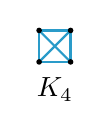
\begin{tikzpicture}[scale=0.4, baseline=(current bounding box.center)]
        \coordinate (a) at (0,0); \coordinate (b) at (1,0);
        \coordinate (c) at (1,1); \coordinate (d) at (0,1);
        \draw[cyan!80!black, thick] (a)--(b)--(c)--(d)--(a);
        \draw[cyan!80!black, thick] (a)--(c); \draw[cyan!80!black, thick] (b)--(d);
        \foreach \p in {a,b,c,d} \filldraw (\p) circle (2pt);
        \node[below] at (0.5,-0.2) {$K_4$};
    \end{tikzpicture}
    \textbf{\color{red}does not even contain} an Eulerian trail.

    \item[7)] Generally, every $K_{2n+1}$ is Eulerian and every $K_{2n+2}$ does not even contain an Eulerian trail for $n \ge 1$.
\end{enumerate}
\end{example}

% 4.3 Observation
\topic{Observation}

Consider the graph $K_5$. We observe the following properties:
\begin{enumerate}
    \item[1)] $K_5$ is Eulerian: $(a,b,c,d,e,a,d,b,e,c,a)$ is an Eulerian circuit.
    \begin{center}
    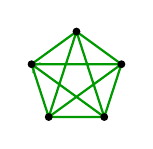
\begin{tikzpicture}[scale=0.6]
        \foreach \i in {1,...,5} \coordinate (v\i) at (90+72*\i:1);
        \foreach \i in {1,...,5} \foreach \j in {\i,...,5} \draw[cyan!20, thin] (v\i)--(v\j);
        \draw[green!60!black, thick, ->] (v1)--(v2)--(v3)--(v4)--(v5)--(v1)--(v4)--(v2)--(v5)--(v3)--(v1);
        \foreach \i in {1,...,5} \filldraw (v\i) circle (2pt);
    \end{tikzpicture}
    \end{center}

    \item[2)] Every vertex of $K_5$ has an even degree. (All 4).
    \begin{center}
    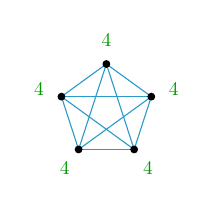
\begin{tikzpicture}[scale=0.6]
        \foreach \i in {1,...,5} \coordinate (v\i) at (90+72*\i:1);
        \foreach \i in {1,...,5} \foreach \j in {\i,...,5} \draw[cyan!80!black] (v\i)--(v\j);
        \foreach \i in {1,...,5} \filldraw (v\i) circle (2pt) node[anchor=center, shift={(90+72*\i:0.3)}, scale=0.7, green!60!black] {4};
    \end{tikzpicture}
    \end{center}
    
    \item[3)] We can partition $E_{K_5}$ into cycles (i.e. find mutually edge-disjoint cycles that together use all edges of $K_5$).
    
    \vspace{0.3cm}
    
    \begin{minipage}[t]{0.45\textwidth}
        \centering
        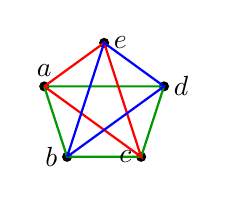
\begin{tikzpicture}[scale=0.8]
            \foreach \i in {1,...,5} \coordinate (v\i) at (90+72*\i:1);
            \foreach \i in {1,...,5} \filldraw (v\i) circle (2pt);
            
            % Decomposition 1: C1(green), C2(red), C3(blue)
            \draw[green!60!black, thick] (v1)--(v2)--(v3)--(v4)--(v1); % 4-cycle
            \draw[red, thick] (v1)--(v3)--(v5)--(v1); % Triangle
            \draw[blue, thick] (v2)--(v4)--(v5)--(v2); % Triangle
            
            \node[above] at (v1) {$a$}; \node[left] at (v2) {$b$}; \node[left] at (v3) {$c$};
            \node[right] at (v4) {$d$}; \node[right] at (v5) {$e$};
        \end{tikzpicture}
        \\
        {\color{green!60!black}$C_1=(a,b,c,d)$} \\
        {\color{red}$C_2=(a,c,e)$} \\
        {\color{blue}$C_3=(b,d,e)$}
    \end{minipage}
    \textbf{or}
    \begin{minipage}[t]{0.45\textwidth}
        \centering
        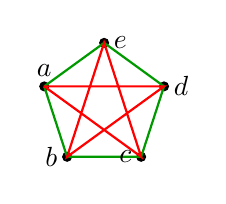
\begin{tikzpicture}[scale=0.8]
            \foreach \i in {1,...,5} \coordinate (v\i) at (90+72*\i:1);
            \foreach \i in {1,...,5} \filldraw (v\i) circle (2pt);
            
            % Decomposition 2: Two 5-cycles
            \draw[green!60!black, thick] (v1)--(v2)--(v3)--(v4)--(v5)--(v1); % Outer
            \draw[red, thick] (v1)--(v3)--(v5)--(v2)--(v4)--(v1); % Inner star
            
            \node[above] at (v1) {$a$}; \node[left] at (v2) {$b$}; \node[left] at (v3) {$c$};
            \node[right] at (v4) {$d$}; \node[right] at (v5) {$e$};
        \end{tikzpicture}
        \\
        {\color{green!60!black}$C_1=(a,b,c,d,e,a)$} \\
        {\color{red}$C_2=(a,c,e,b,d,a)$}
    \end{minipage}
\end{enumerate}

These three properties do not appear together by coincidence. It turns out, they are equivalent to each other.

% 4.4 Auxiliary Lemma
\begin{lemma}[Auxiliary Lemma]
Let $G$ be a connected graph with $|G| \ge 2$. If $\deg(v)$ is even for all $v \in V_G$, then $G$ contains a cycle $C$. Moreover, $G-C$ still contains a cycle or is $E_{|G|}$.
\end{lemma}

\begin{proof}
Assume $G$ is as above. If $G$ would not contain a cycle, it was a tree. But then it had to contain a leaf $v$. But then $\deg(v)=1$ is not even \textbf{\color{red}$\lightning$}.
For the ``moreover'' part, observe that
\[ \deg^{G-C}(v) = \begin{cases} \deg^G(v)-2 & \text{if } v \in V_C \\ \deg^G(v) & \text{else} \end{cases} \]
hence still even. Then each connected component of $G-C$ still contains a cycle (whence so does $G-C$), or is of order 1.
\end{proof}

% 4.5 Theorem
\begin{theorem}[Euler-Hierholzer-Veblen]
Let $G$ be a connected graph. The following are equivalent:
\begin{enumerate}
    \item[1)] $G$ is Eulerian.
    \item[2)] Every vertex of $G$ is of even degree.
    \item[3)] The edge set of $G$ can be partitioned into a set of edge-disjoint cycles.
\end{enumerate}
\end{theorem}

% 4.6 Corollary
\begin{corollary}
A graph contains an Eulerian trail iff either each vertex has even degree or there are exactly two vertices of odd degree.
\end{corollary}

\begin{proof}
Proof of Theorem 4.5:
As all three clearly hold for $|G|=1$, we may assume that $|G|>1$.

\underline{$1) \Rightarrow 2)$}: Assume $G$ is Eulerian. Let $Q$ be an Eulerian circuit of $G$. Now consider $v \in V_G$ arbitrary. Without loss of generalisation, we may assume that $Q$ does not start with $v$. Now, every appearence of $v$ in $Q$ corresponds to two distinct edges involving $v$, the one leading \textit{into} $v$ and the one leading \textit{away} from $v$. As $Q$ is Eulerian, it uses all edges incident with $v$ whence in total there is an even number of edges incident with $v$ and $\deg(v)$ is even. \checkmark

\underline{$2) \Rightarrow 3)$}: Assume $G$ only contains vertices of even degree. By Lemma 4.4, $G$ contains at least one cycle $C$. We proceed by induction on the number $n$ of cycles in $C$.
\textbf{n=1}: If $G$ contains only one cycle, then $G=C_{|G|}$ and hence the desired partition of edges is just the cycle $G$ itself.
\textbf{n $\to$ n+1}: Now assume every graph containing at most $n$-many cycles allows a partition into edge-disjoint cycles. Consider any connected $G$ with $(n+1)$-many cycles. Pick an arbitrary cycle $C$ in $G$. Then as in 4.4, in $H := (V_G, E_G - E_C)$, every vertex still has even degree. Now, every connected component of $H$ contains at most $n$-many cycles. By induction hypothesis, we can partition each connected component of $H$, and hence $H$ itself, into edge-disjoint cycles. Once we add $C$ to this partition, we obtain the desired partition of $G$. \checkmark (Note that this gives you a cooking recipe of how to find cycles).

\underline{$3) \Rightarrow 1)$}: Assume the edge set of $G$ can be partitioned into $k$-many sets $S_1, S_2, \dots, S_k$ s.t. the edges of each $S_i$ form a cycle.
Let $Q$ be a circuit of maximal length in $G$ s.t. the edges of $Q$ equals the union of some sets $S_i$, i.e. such that there is $I \subseteq \{1, \dots, k\}$ with $E_Q = \bigcup_{i \in I} S_i$.
As the $S_i$ are pairwise disjoint, we know that $Q$ contains either no edge from $S_i$ or all edges from $S_i$ for every $i \le k$.
Now, if $E_Q = E_G$, then $G$ is Eulerian and we are done.
Otherwise, there is some edge not contained in $Q$, but incident with a vertex $v$ in $Q$. The edge must be contained in exactly one $S_\ell$ with $\ell \notin I$. Note that $Q$ and $S_\ell$ have no common edges, but they share the vertex $v$. Hence we may glue the circuit $Q$ and the cycle $S_\ell$ at $v$ and obtain a new circuit $Q'$ longer than $Q$ with $E_{Q'} = \bigcup_{i \in I \cup \{\ell\}} S_i$, contradicting our choice of $Q$.
Hence $Q$ contained all edges of $G$ and hence $G$ is Eulerian. \checkmark
\end{proof}

\section{Hamilton}

\textbf{Sir William Rowan Hamilton (1805--1865)}
\begin{itemize}
    \item Irish pure mathematician
    \item Contributions to optics, mechanics and algebra.
    \item Also invented a game (The Icosian Game) build on graph theory (bought by Jaques and Son, huge failure).
\end{itemize}

% 4.7 Definition
\begin{definition}
Let $G$ be a graph. A \textbf{\color{red}Hamiltonian path} is a path in $G$ which uses all vertices of $G$. A \textbf{\color{red}Hamiltonian cycle} is a cycle in $G$ which uses all of $V_G$.
We call $G$ \textbf{\color{red}traceable} if it contains a Hamiltonian path and we call it \textbf{\color{red}Hamiltonian} if it contains a Hamiltonian cycle.
\end{definition}

% 4.8 Remark
\begin{remark}
\begin{enumerate}
    \item[1)] Every Hamiltonian graph is traceable but not vice versa.
    \item[2)] Traceable graphs are connected.
    \item[3)] If $|G|=n$, then $G$ is Hamiltonian iff it contains $C_n$ as a subgraph and it is traceable iff it contains $P_n$ as a subgraph.
\end{enumerate}
\end{remark}

% 4.9 Examples
\begin{example}
\begin{enumerate}
    % Item 1: C6
    \item 
    \begin{minipage}[t]{0.6\textwidth}
        $C_6$ \textbf{\color{green!60!black}is Hamiltonian} via $v_1 \dots v_6 v_1$. \\
        {\color{blue!80!black}\small All vertices have even degree.}
    \end{minipage}
    \begin{minipage}[t]{0.3\textwidth}
        \centering
        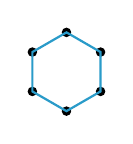
\begin{tikzpicture}[scale=0.5, baseline=(current bounding box.north)]
            \foreach \i in {1,...,6} \filldraw (90+60-60*\i:1) circle (3pt);
            \draw[cyan!80!black, thick] (90:1) -- (30:1) -- (-30:1) -- (-90:1) -- (210:1) -- (150:1) -- cycle;
        \end{tikzpicture}
    \end{minipage}

    % Item 2: K4
    \item 
    \begin{minipage}[t]{0.6\textwidth}
        $K_4$ \textbf{\color{green!60!black}is Hamiltonian} via $v_1 v_2 v_3 v_4 v_1$. \\
        {\color{blue!80!black}\small All vertices have odd degree.}
    \end{minipage}
    \begin{minipage}[t]{0.3\textwidth}
        \centering
        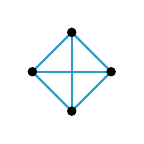
\begin{tikzpicture}[scale=0.5, baseline=(current bounding box.north)]
            \coordinate (a) at (0,1); \coordinate (b) at (1,0);
            \coordinate (c) at (0,-1); \coordinate (d) at (-1,0);
            \draw[cyan!80!black, thick] (a)--(b)--(c)--(d)--(a);
            \draw[cyan!80!black, thick] (a)--(c); \draw[cyan!80!black, thick] (b)--(d);
            \foreach \p in {a,b,c,d} \filldraw (\p) circle (3pt);
        \end{tikzpicture}
    \end{minipage}

    % Item 3: G1 (Wheel graph)
    \item 
    \begin{minipage}[t]{0.6\textwidth}
        The graph $G_1$ \textbf{\color{green!60!black}is Hamiltonian}. \\
        {\color{blue!80!black}\small There are vertices of even and odd degree.}
    \end{minipage}
    \begin{minipage}[t]{0.3\textwidth}
        \centering
        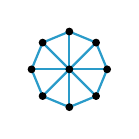
\begin{tikzpicture}[scale=0.4, baseline=(current bounding box.north)]
            \coordinate (c) at (0,0);
            \foreach \i in {1,...,8} \coordinate (v\i) at (90+45-45*\i:1.2);
            \draw[cyan!80!black, thick] (v1)--(v2)--(v3)--(v4)--(v5)--(v6)--(v7)--(v8)--(v1);
            \foreach \i in {1,...,8} \draw[cyan!80!black, thick] (c)--(v\i);
            \foreach \i in {1,...,8} \filldraw (v\i) circle (3pt); \filldraw (c) circle (3pt);
        \end{tikzpicture}
    \end{minipage}

    % Item 4: G2 (Two squares sharing a vertex)
    \item 
    \begin{minipage}[t]{0.6\textwidth}
        The graph $G_2$ is \textbf{not} Hamiltonian. \\
        {\color{blue!80!black}\small Every vertex has even degree.}
    \end{minipage}
    \begin{minipage}[t]{0.3\textwidth}
        \centering
        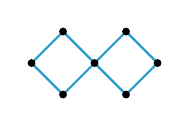
\begin{tikzpicture}[scale=0.4, baseline=(current bounding box.north)]
            % Two diamonds touching
            \coordinate (c) at (0,0);
            \coordinate (t1) at (-1,1); \coordinate (b1) at (-1,-1); \coordinate (l1) at (-2,0);
            \coordinate (t2) at (1,1); \coordinate (b2) at (1,-1); \coordinate (r2) at (2,0);
            
            % Left diamond
            \draw[cyan!80!black, thick] (c)--(t1)--(l1)--(b1)--(c);
            % Right diamond
            \draw[cyan!80!black, thick] (c)--(t2)--(r2)--(b2)--(c);
            
            \foreach \p in {c,t1,b1,l1,t2,b2,r2} \filldraw (\p) circle (3pt);
        \end{tikzpicture}
    \end{minipage}

    % Item 5: K1,3
    \item 
    \begin{minipage}[t]{0.6\textwidth}
        The graph $K_{1,3}$ is \textbf{not} Hamiltonian. \\
        {\color{blue!80!black}\small All vertices have odd degree.}
    \end{minipage}
    \begin{minipage}[t]{0.3\textwidth}
        \centering
        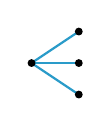
\begin{tikzpicture}[scale=0.4, baseline=(current bounding box.north)]
            \coordinate (c) at (0,0);
            \coordinate (r1) at (1.5, 1); \coordinate (r2) at (1.5, 0); \coordinate (r3) at (1.5, -1);
            \draw[cyan!80!black, thick] (c)--(r1); \draw[cyan!80!black, thick] (c)--(r2); \draw[cyan!80!black, thick] (c)--(r3);
            \foreach \p in {c,r1,r2,r3} \filldraw (\p) circle (3pt);
        \end{tikzpicture}
    \end{minipage}

    % Item 6: P4
    \item 
    \begin{minipage}[t]{0.6\textwidth}
        The path $P_4$ is \textbf{not} Hamiltonian. \\
        {\color{blue!80!black}\small There are vertices of even and odd degree.}
    \end{minipage}
    \begin{minipage}[t]{0.3\textwidth}
        \centering
        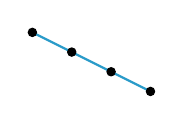
\begin{tikzpicture}[scale=0.5, baseline=(current bounding box.north)]
            \foreach \i in {0,1,2,3} \coordinate (p\i) at (\i, -0.5*\i); % Slanted path
            \draw[cyan!80!black, thick] (p0)--(p1)--(p2)--(p3);
            \foreach \i in {0,1,2,3} \filldraw (p\i) circle (3pt);
        \end{tikzpicture}
    \end{minipage}
\end{enumerate}
\end{example}

% 4.10 Remark
\begin{remark}
While it is rather easy to decide whether a graph is Eulerian (P-TIME, $O(|G|^2)$), it is surprisingly \textbf{hard} to do the same for Hamiltonian graphs. This problem is known to be \textbf{NP-complete} and still we did not manage to find an equivalent condition for Hamiltonianity (other than containing $C_{|G|}$ as a subgraph, which is basically the definition).

We hence see, even though the Eulerian graph problem and the Hamiltonian graph problem seem so similar, their resolution requires very different levels of efforts.
The best we can do at the moment is give some \textbf{sufficient} criteria.
\end{remark}

% 4.11 Theorem
\begin{theorem}[Dirac]
Let $G$ be s.t. $|G| \ge 3$. If $\delta(G) \ge \frac{n}{2}$, then $G$ is Hamiltonian.
\end{theorem}

\begin{proof}
Consider $G$ arbitrary s.t. $|G|=n \ge 3$ and $\delta(G) \ge \frac{n}{2}$.\\
Then $G$ is necessarily connected (think why).\\
Consider a path $P=(v_1, v_2, \dots, v_k)$ of maximal length in $G$.\\
We claim that there is some $j < k$ s.t. $v_{j+1} \in N(v_1)$ and $v_j \in N(v_k)$. i.e.
\begin{center}
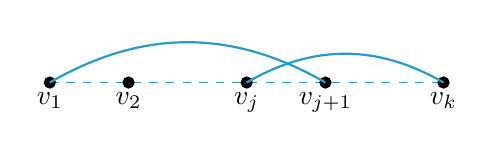
\begin{tikzpicture}[scale=1]
    % Path
    \draw[cyan!80!black, dashed] (0,0) -- (5,0);
    \foreach \x/\l in {0/v_1, 1/v_2, 2.5/v_j, 3.5/v_{j+1}, 5/v_k} \filldraw (\x,0) circle (2pt) node[below] {$\l$};
    % Cross edges
    \draw[cyan!80!black, thick] (0,0) to[bend left] (3.5,0);
    \draw[cyan!80!black, thick] (2.5,0) to[bend left] (5,0);
\end{tikzpicture}
\end{center}
is a subgraph of $P$. Note that as usual, as $P$ is of maximal length, all neighbours of $v_1$ and $v_k$ must be on $P$. As $\delta(G) \ge \frac{n}{2}$, $v_k$ has at least $\frac{n}{2}$ many neighbours $v_j$ in $P$. Aiming for a contradiction, assume for every neighbour $v_j \in N(v_k)$, $v_{j+1} \notin N(v_1)$. Then there are at least $\frac{n}{2}$ many vertices in $P$ which are \textbf{not} neighbours of $v_1$. This now yields the desired contradiction, as all neighbours of $v_1$ are on $P$ and thus $\deg(v_1) \le (k-1) - \frac{n}{2} \le (n-1) - \frac{n}{2} = \frac{n}{2} - 1 < \frac{n}{2}$, contradicting $\delta(G) \ge \frac{n}{2}$.
Hence there is some $j$ s.t. $v_1 v_{j+1}$ and $v_j v_k$ are edges, which leads to the existence of a cycle
\[ C = (v_1, v_2, \dots, v_j, v_k, v_{k-1}, \dots, v_{j+1}, v_1). \]
\begin{center}
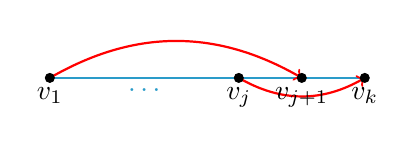
\begin{tikzpicture}[scale=0.8]
    % Visualizing the Posa rotation cycle
    \draw[cyan!80!black, thick] (0,0)--(1,0)--(2,0) node[midway, below] {$\dots$}--(3,0)--(4,0)--(5,0);
    \draw[red, thick, ->] (0,0) to[bend left] (4,0);
    \draw[red, thick, ->] (3,0) to[bend right] (5,0);
    \filldraw (0,0) circle (2pt) node[below] {$v_1$};
    \filldraw (5,0) circle (2pt) node[below] {$v_k$};
    \filldraw (3,0) circle (2pt) node[below] {$v_j$};
    \filldraw (4,0) circle (2pt) node[below] {$v_{j+1}$};
\end{tikzpicture}
\end{center}
Finally, we claim that $C$ is indeed a Hamiltonian cycle, i.e. it contains all vertices of $G$. Otherwise, as $G$ is connected, there is a vertex $u$ in $G \setminus C$ which is adjacent to one vertex $v_i$ in $C$. But as $C$ is a cycle, we can form a new path starting in $u, v_i \dots$ and then traveling through all $k-1$ many vertices of $C$. This path is longer than $P$, contradicting our choice of $P$.
Hence, $C$ indeed contains all vertices of $G$ whence it is a Hamiltonian cycle and $G$ is Hamiltonian.
\end{proof}

% 4.12 Fact
\begin{theorem}[{Fact - Ore, 1960}]
Let $G$ be a graph of order $n \ge 3$. Suppose for every pair of non-adjacent vertices $u,v$ we have that $\deg(u) + \deg(v) \ge n$. Then $G$ is Hamiltonian.
\end{theorem}

Note that now Dirac's Theorem is a mere corollary of Ore's theorem.\\
We want to achieve yet another sufficient criterion for Hamiltonicity. This leads us to the so-called independence number.

% 4.13 Definition
\begin{definition}
Let $G$ be a graph. A set $S \subseteq V_G$ of vertices is called an \textbf{\color{red}independent set} if any two vertices in $S$ are nonadjacent.
The \textbf{\color{red}independence number $\alpha(G)$} of $G$ is the maximal size of an independent set.
\end{definition}

% 4.14 Examples
\begin{example}
\begin{itemize}
    \item $\alpha(E_n) = n$, as $V_{E_n}$ is an independent set.
    \item $\alpha(K_n) = 1$, as any two vertices are adjacent. Actually, the converse also holds, i.e. $\alpha(G)=1$ iff $G$ is complete.
    \item $\alpha(K_{n,m}) = \max\{n,m\}$, as any set is independent iff it is contained in one of the parts.
\end{itemize}
\end{example}

% 4.15 Notation
\topic{Notation}
If $P$ is a path and $x,y$ are two vertices on $P$, then we denote by \textbf{\color{red}$P[x,y]$} the subpath on $P$ from $x$ to $y$. E.g. for
\begin{center}
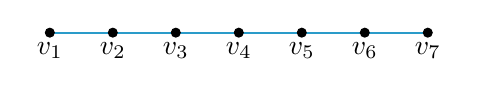
\begin{tikzpicture}[scale=0.8]
    % Path v1 to v7
    \draw[cyan!80!black, thick] (0,0) -- (6,0);
    \foreach \i in {1,...,7} \filldraw (\i-1, 0) circle (2pt) node[below] {$v_\i$};
\end{tikzpicture}
\end{center}
we have $P[v_6, v_3] = (v_6, v_5, v_4, v_3)$.

Similarly, if $C$ is a cycle and $x,y \in C, x \neq y$, then we denote by \textbf{\color{red}$C^+[x,y]$} the $xy$-path on $C$ in clockwise direction and by \textbf{\color{red}$C^-[x,y]$} the $xy$-path on $C$ in counter-clockwise direction.

E.g. if $C$ is
\begin{center}
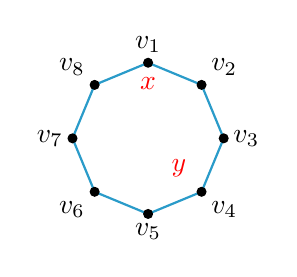
\begin{tikzpicture}[scale=0.8, baseline=(current bounding box.center)]
    % Octagon C8
    \foreach \i in {1,...,8} \coordinate (v\i) at (90+45-45*\i : 1.2);
    \draw[cyan!80!black, thick] (v1)--(v2)--(v3)--(v4)--(v5)--(v6)--(v7)--(v8)--(v1);
    
    \foreach \i in {1,...,8} \filldraw (v\i) circle (2pt);
    
    % Labels v1..v8
    \node[above] at (v1) {$v_1$}; \node[above right] at (v2) {$v_2$};
    \node[right] at (v3) {$v_3$}; \node[below right] at (v4) {$v_4$};
    \node[below] at (v5) {$v_5$}; \node[below left] at (v6) {$v_6$};
    \node[left] at (v7) {$v_7$}; \node[above left] at (v8) {$v_8$};

    % Red markers x and y (x at v1, y at v4 based on notes)
    \node[red, below=2pt] at (v1) {$x$};
    \node[red, above left=2pt] at (v4) {$y$};
\end{tikzpicture}
\end{center}
then $C^+[x,y] = (v_1, v_2, v_3, v_4)$ and $C^-[x,y] = (v_1, v_8, v_7, v_6, v_5, v_4)$.

Finally, for sequences $s=(x_1, \dots, x_\ell), t=(y_1, \dots, y_k)$ we define \textbf{\color{red}$s \hat{\ } t$} $:= (x_1, \dots, x_\ell, y_1, \dots, y_k)$ to be the concatenation of both.

% 4.16 Theorem
% 4.16 Theorem
\begin{theorem}[{Chv\'atal, Erd\H{o}s, 1972}]
Let $G$ be a graph of order at least 3. If $\kappa(G) \ge \alpha(G)$, then $G$ is Hamiltonian.
\end{theorem}

\begin{proof}
Let $G$ be as above, i.e. $|G| \ge 3, \kappa(G) \ge 1, \kappa(G) \ge \alpha(G)$.
\begin{itemize}
    \item First we argue that $\kappa(G) \ge 2$. Otherwise $\kappa(G)=\alpha(G)=1$, whence $G$ is a complete graph. As further $\kappa(K_n)=n-1$, $G$ would be $K_2$, contradicting $|G| \ge 3$.
    \item Hence now we know that $\kappa(G) \ge 2$. By 1.41(8), we know that $\delta(G) \ge \kappa(G) \ge 2$, whence by 1.39, $G$ contains a cycle.
\end{itemize}

Now consider a cycle $C$ of maximal length in $C$. We claim that $C$ is Hamiltonian.
Aiming for a contradiction, assume $C$ is not Hamiltonian, i.e. there is some vertex $v \notin C$.
Let $H$ be the connected component of $v$ in $G \setminus C$.

\begin{center}
    \includegraphics[width=0.6\textwidth]{./images/pic_4_16_1.png} % Placeholder 1: Setup Diagram (H and C)
\end{center}

Now, we list all elements of $C$ which are connected to some vertex in $H$ in clockwise order: $\{c_1, c_2, \dots, c_r\}$ (s.t. $c_j \in C^+[c_{j-1}, c_{j+1}]$), i.e. where each $c_i$ is adjacent to some $h_i \in H$.

\begin{center}
    \includegraphics[width=0.6\textwidth]{./images/pic_4_16_2.png} % Placeholder 2: c_i definition diagram
\end{center}

\textbf{Claim 1:} No two $c_i$'s are consecutive vertices in $C$.
Proof: Otherwise assume there is an $i$ s.t. $c_{i+1}$ is the clockwise successor of $c_i$. Let $P$ be a path from $h_i$ to $h_{i+1}$ in $H$.
Then $C^+[c_{i+1}, c_i] \hat{\ } (c_i h_i) \hat{\ } P \hat{\ } (h_{i+1} c_{i+1})$ is a cycle strictly longer than $C$, contradicting our assumptions. $\lightning$

\begin{center}
    \includegraphics[width=0.6\textwidth]{./images/pic_4_16_3.png} % Placeholder 3: Claim 1 contradiction diagram
\end{center}

Now that no two $c_i$ and $c_j$ are clockwise successors, we can define the set $D = \{d_1, d_2, \dots, d_r\}$ where each $d_i$ is the clockwise successor of $c_i$ in $C$ and we get that $\{c_1, \dots, c_r\} \cap \{d_1, \dots, d_r\} = \emptyset$.

\begin{center}
    \includegraphics[width=0.6\textwidth]{./images/pic_4_16_4.png} % Placeholder 4: Definition of d_i diagram
\end{center}

\textbf{Claim 2:} $\{c_1, \dots, c_r\}$ is a cut set for $G$.
Proof: This is clear as any path from $v$ to a vertex in $C$ has to pass through one of the vertices in $\{c_1, \dots, c_r\}$, so $G - \{c_1, \dots, c_r\}$ is disconnected.
Consequently, as $\kappa(G)$ is the size of a smallest cut set, we obtain that $r \ge \kappa(G) \ge 2$.

\textbf{Claim 3:} There are $d_i$ and $d_j$ which are adjacent.
Proof: Consider the set $X := \{d_1, d_2, \dots, d_r, v\}$, and recall that there is no edge between any $d_i$ and $v$. As $|X| = r+1 \ge \kappa(G)+1 > \alpha(G)$, $X$ cannot be an independent set, whence at least one pair $d_i, d_j$ must be adjacent.

\begin{center}
    \includegraphics[width=0.6\textwidth]{./images/pic_4_16_5.png} % Placeholder 5: Claim 3 / Edge d_i d_j diagram
\end{center}

Now we are ready for our final contradiction: We produce a cycle $\hat{C}$ longer than $C$. Assume $d_i d_j$ is an edge and $i < j$. Let $q_{h_i h_j}$ be a path in $H$ from $h_i$ to $h_j$.
Now define $\hat{C} = (c_i) \hat{\ } q_{h_i h_j} \hat{\ } (c_j) \hat{\ } C^-[c_j, d_i] \hat{\ } (d_i d_j) \hat{\ } C^+[d_j, c_i]$.

\begin{center}
    \includegraphics[width=0.6\textwidth]{./images/pic_4_16_6.png} % Placeholder 6: Final Cycle Construction diagram
\end{center}

Note that $\hat{C}$ uses all edges of $C$ except the edges $c_i d_i$ and $c_j d_j$. Instead it uses at least the three additional edges $c_i h_i, h_j c_j$ and $d_i d_j$. Hence, $\hat{C}$ is strictly longer than the cycle $C$, which contradicts our choice of $C$.
Conclusively, $C$ must contain all vertices of $G$ and hence is Hamiltonian.
\end{proof}

So far, we have encountered sufficient criteria for Hamiltonian graphs using the degree of vertices and the independence number. We will conclude the chapter by providing a last sufficient criterium using a new concept - \textbf{\color{red}forbidden subgraphs}.

% 4.17 Definition
\begin{definition}
Let $H$ and $G$ be graphs. We say that $G$ is \textbf{\color{red}$H$-free} if $H$ is not (isomorphic to) an induced subgraph of $G$. Moreover, if $S$ is a collection of graphs, then we call $G$ \textbf{\color{red}$S$-free} iff $G$ is $H$-free for any $H \in S$.
\end{definition}

% 4.18 Example
\begin{example}
The Petersen graph
\begin{center}
\begin{tikzpicture}[scale=0.85]
    % --- Left Text Block with Brace ---
    \node[anchor=east] at (-3, 0) {
        $\begin{aligned}
            & \text{is \textbf{\color{green!60!black}indeed} } C_3\text{-free} \\
            & \text{is \textbf{\color{red}not} } C_5\text{-free} \\
            & \text{is \textbf{\color{red}not} } E_4\text{-free} \\
            & \text{is \textbf{\color{green!60!black}indeed} } E_5\text{-free}
        \end{aligned}
        \left\} \parbox{0.5cm}{\vspace{2cm}} \right.$ % Invisible parbox to stretch the brace
    };

    % --- Center: The Graph G ---
    \node at (-2, 0.5) {$G=$};
    \begin{scope}[xshift=0cm]
        % Outer pentagon
        \foreach \i in {1,...,5} \coordinate (o\i) at (90+72*\i:1.5);
        % Inner star
        \foreach \i in {1,...,5} \coordinate (i\i) at (90+72*\i:0.7);
        
        \draw[cyan!80!black, thick] (o1)--(o2)--(o3)--(o4)--(o5)--(o1);
        \draw[cyan!80!black, thick] (i1)--(i3)--(i5)--(i2)--(i4)--(i1);
        \foreach \i in {1,...,5} \draw[cyan!80!black, thick] (o\i)--(i\i);
        \foreach \p in {o1,o2,o3,o4,o5,i1,i2,i3,i4,i5} \filldraw (\p) circle (2pt);
    \end{scope}

    % --- Right: Recall Info ---
    \node[anchor=west, align=left, blue!80!black, scale=0.9] at (2, 0.5) {
        Recall: \\
        $\kappa(G)=3$ \\
        $\alpha(G)=4$
    };

    % --- Bottom Text ---
    \node[anchor=west] at (2, -1) {
        $G$ is hence also $\{C_3, E_5\}$-free.
    };
\end{tikzpicture}
\end{center}
\end{example}

% 4.19 Notations
\topic{Notations}

Let $Z_1$ be the graph $Z_1 =$ 
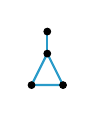
\begin{tikzpicture}[baseline=-0.5ex, scale=0.4]
    % Triangle with top antenna
    \coordinate (a) at (-0.5,-0.5); \coordinate (b) at (0.5,-0.5); \coordinate (c) at (0,0.5);
    \coordinate (d) at (0,1.2);
    \draw[cyan!80!black, thick] (a)--(b)--(c)--(a);
    \draw[cyan!80!black, thick] (c)--(d);
    \foreach \p in {a,b,c,d} \filldraw (\p) circle (3pt);
\end{tikzpicture}
and $N=$
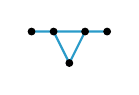
\begin{tikzpicture}[baseline=-0.5ex, scale=0.4]
    % Triangle with side legs
    \coordinate (a) at (-0.5,0.5); \coordinate (b) at (0.5,0.5); \coordinate (c) at (0,-0.5);
    \coordinate (l) at (-1.2, 0); \coordinate (r) at (1.2, 0);
    % Actually looking at notes N: Triangle base, two legs out
    \draw[cyan!80!black, thick] (a)--(b)--(c)--(a);
    \draw[cyan!80!black, thick] (a)--(-1.2, 0.5);
    \draw[cyan!80!black, thick] (b)--(1.2, 0.5);
    \filldraw (a) circle (3pt); \filldraw (b) circle (3pt); \filldraw (c) circle (3pt);
    \filldraw (-1.2, 0.5) circle (3pt); \filldraw (1.2, 0.5) circle (3pt);
\end{tikzpicture}.

Further, we call the graph $K_{1,3}$ the \textbf{\color{red}claw}, based on its shape:
$K_{1,3} =$ 

\begin{tikzpicture}[baseline=-0.5ex, scale=0.4]
    % Claw shape 1: <
    \coordinate (c) at (0.5,0);
    \draw[cyan!80!black, thick] (c)--(0, 0.5);
    \draw[cyan!80!black, thick] (c)--(-0.2, 0);
    \draw[cyan!80!black, thick] (c)--(0, -0.5);
    \filldraw (c) circle (3pt); \filldraw (0,0.5) circle (3pt); \filldraw (-0.2,0) circle (3pt); \filldraw (0,-0.5) circle (3pt);
\end{tikzpicture}
, or also $K_{1,3} =$ 
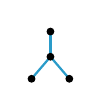
\begin{tikzpicture}[baseline=-0.5ex, scale=0.4]
    % Claw shape 2: Y (Mercedes star)
    \coordinate (c) at (0,0.2);
    \draw[cyan!80!black, thick] (c)--(0, 1);
    \draw[cyan!80!black, thick] (c)--(-0.6, -0.5);
    \draw[cyan!80!black, thick] (c)--(0.6, -0.5);
    \filldraw (c) circle (3pt); \filldraw (0,1) circle (3pt); \filldraw (-0.6,-0.5) circle (3pt); \filldraw (0.6,-0.5) circle (3pt);
\end{tikzpicture}.
\\
\\
% 4.20 Theorem
\begin{theorem}[{Goodman, Hedetniemi, 1974}]
Let $G$ be 2-connected and $\{K_{1,3}, Z_1\}$-free, then $G$ is Hamiltonian.
\end{theorem}

\begin{proof}
As $\delta(G) \ge \kappa(G) \ge 2$, we get that $G$ contains a cycle. Consider such a cycle $C$ of maximal length. We claim that $C$ is Hamiltonian.\\
Otherwise, as $G$ is connected, there was a vertex $v \in V_G$ not on $C$ but adjacent to some vertex $x$ on $C$, i.e.
\begin{center}
    \includegraphics[width=0.6\textwidth]{./images/pic_4_20.png} % Placeholder 1: Setup Diagram (H and C)
\end{center}
Denote by $y$ and $z$ the neighbours of $x$ on $C$.\\
Note that $yv$ is not an edge as otherwise replacing the subsequence $(y,x)$ in $C$ by $(y,v,x)$ would yield a cycle longer than $C$. Similarly, $vz$ is not an edge.
Consequently, the induced subgraph on $S=\{x,y,z,v\}$ is either
$\langle S \rangle = K_{1,3}$ 
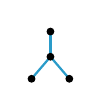
\begin{tikzpicture}[baseline=-0.5ex, scale=0.4]
    % Claw shape 2: Y (Mercedes star)
    \coordinate (c) at (0,0.2);
    \draw[cyan!80!black, thick] (c)--(0, 1);
    \draw[cyan!80!black, thick] (c)--(-0.6, -0.5);
    \draw[cyan!80!black, thick] (c)--(0.6, -0.5);
    \filldraw (c) circle (3pt); \filldraw (0,1) circle (3pt); \filldraw (-0.6,-0.5) circle (3pt); \filldraw (0.6,-0.5) circle (3pt);
\end{tikzpicture} or $\langle S \rangle = Z_1$, 
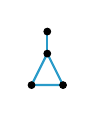
\begin{tikzpicture}[baseline=-0.5ex, scale=0.4]
    % Triangle with top antenna
    \coordinate (a) at (-0.5,-0.5); \coordinate (b) at (0.5,-0.5); \coordinate (c) at (0,0.5);
    \coordinate (d) at (0,1.2);
    \draw[cyan!80!black, thick] (a)--(b)--(c)--(a);
    \draw[cyan!80!black, thick] (c)--(d);
    \foreach \p in {a,b,c,d} \filldraw (\p) circle (3pt);
\end{tikzpicture} both of which contradict our assumptions on $G$.
\end{proof}

The following final condition is now easy to verify:

% 4.21 Theorem
\begin{theorem}[{Duffus, Gould, Jacobson, 1980}]
Let $G$ be a $\{K_{1,3}, N\}$-free graph.\\
i) If $G$ is connected, it is traceable.\\
ii) If $G$ is 2-connected, it is Hamiltonian.
\end{theorem}

Note that neither of these are necessary for $G$ to be Hamiltonian. Indeed, for any graph $H$ there is a Hamiltonian graph $G$ which contains $H$ as an induced subgraph.